% c'est compliqué - trop de mikmak tue le mikmak %%%
\documentclass[usenames,dvipsnames, 12pt]{beamer}
\usepackage[frenchb]{babel}
\usepackage[T1]{fontenc}
\usepackage[utf8]{inputenc}
\usepackage{lmodern}
\mode<presentation>

\usepackage{xcolor}
\usetheme{Malmoe}
\usecolortheme{spruce}
\setbeamertemplate{itemize item}{\color{Green}$\bullet$}
\setbeamertemplate{enumerate item}{\color{Green}}
\setbeamertemplate{blocks}[rounded][shadow=trued]
\title{Ma présentation \\avec la classe Beamer de \LaTeX}
\author{William Rapuc}
\institute{EDYTEM}
\date{23 Janvier 2018}


\begin{document}
%%%%%%%%%%%%%%%%%%%%%%%%%%%%%%%%%%%%%%%%%%%%%%%%%%%%%%%
%%%%%%%%%%%%%%%%%%%%%%%%%%%%%%%%%%%%%%%%%%%%%%%%%%%%%%%%%
\section{Introduction}
\subsection{Pingouin}

 \begin{frame}
 \titlepage
 \end{frame}
 \begin{frame}{Titre }{Sous-titre}
  Finalement ce n'est pas si difficile ! Bon pour arriver jusqu'à une présentationc collective on a quand même un peu galéré, admettons!
  	\end{frame}
%%%%%%%%%%%%%%%%%%%%%%%%%%%%%%%%%%%%%%%%%%%%%%%%%%%%%%%
 \subsection{Pingouin 2}
 \begin{frame}{La glisse de Pingouin}{Sous-titre}
 \setbeamercolor{block title}{use=structure,fg=white,bg=ForestGreen!75!black}
\setbeamercolor{block body}{use=structure,fg=black,bg=white!20!white}
	\begin{columns}	
	\column{.5\textwidth}
	\begin{center}
		Bouhou
	\end{center}
	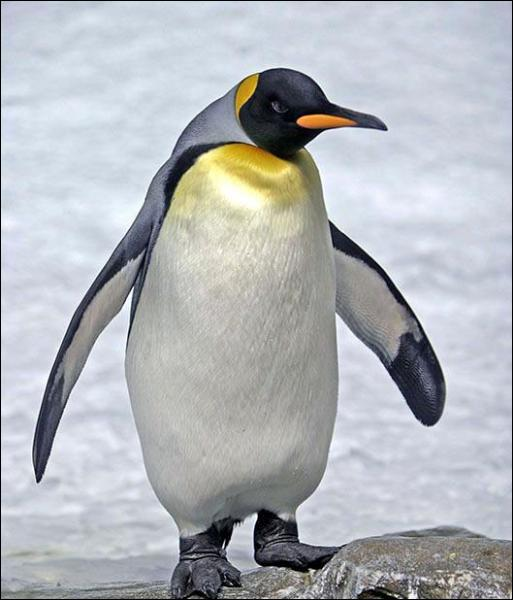
\includegraphics[angle = 90, width = 1.\textwidth]{Pingouin}
	
	\column{.5\textwidth}
  Finalement ce n'est pas si difficile !
  		\begin{block}{Des choses}
  			\begin{itemize}
  			\item<1-3>	une chose
  			\item<2>	une autre
  			\item<3>	une troisième
  			\end{itemize}
  		\end{block}
  		\end{columns}
 \end{frame}
%%%%%%%%%%%%%%%%%%%%%%%%%%%%%%%%%%%%%%%%%%%%%%%%%%
\section{Point de vue}
\subsection{Pingouin 3}
 \begin{frame}{La glisse de Pingouin}{Sous-titre}
 \setbeamercolor{block title}{use=structure,fg=white,bg=ForestGreen!75!black}
\setbeamercolor{block body}{use=structure,fg=black,bg=white!20!white}
	\begin{columns}	
	\column{.5\textwidth}
	\begin{center}
		houBou
	\end{center}
	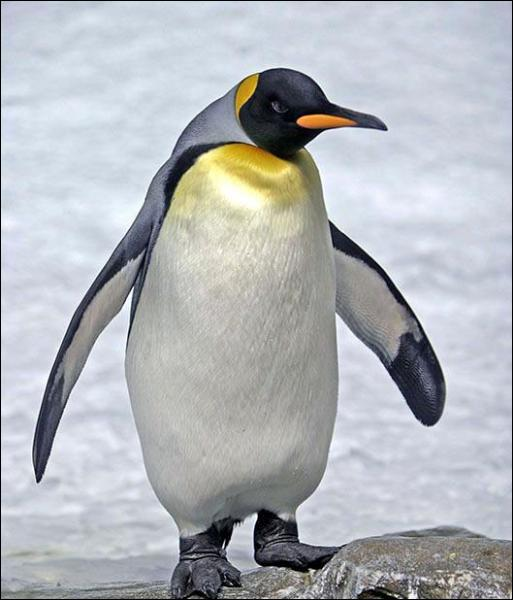
\includegraphics[angle = 180, width = .8\textwidth]{Pingouin}
	
	\column{.5\textwidth}
  		\begin{block}{Des choses}
  			\begin{enumerate}
  			\item	une chose
  			\item	une autre
  			\item	une troisième
  			\end{enumerate}
  		\end{block}
  		\end{columns}
 \end{frame}
%%%%%%%%%%%%%%%%%%%%%%%%%%%%%%%%%%%%%%%%%%%%%%%%%%%%%%%% 
\end{document}
